\subsection{Verwendung der internen ADCs}
\subsubsection{Projektteilbereich Übersicht}
Die im DE10-Lite Board integrierten ADCs werden versucht am Anfang des Projektes anzusteuern und vorläufig, bevor ein Piggyback mit einem externen ADC vorhanden ist, zu verwenden. \textbf{Dieser erste Schritt ist fehlgeschlagen, da die Verwendung der ADCs nur mit einem eingebetteten Nios-Prozessor möglich ist.} Die Implementierung eines solchen komplexen Bausteins würde die zeitlichen Grenzen maßlos überschreiten und ist auch nicht Ziel des Projekts. Die geleistete Arbeit ist trotzdem dokumentiert und auf den folgenden Seiten enthalten.\newline Das Board hat 6 integrierte ADCs. Diese sind mit einer Bandbreite von 12 Bit und einer Sampling-Frequenz von 10 MHz spezifiziert und haben eine Verstärkerschaltung vorgeschalten. Eine analoge Eingangsspannung von 0-5V ist zulässig. Quartus-Prime bietet bereits fertige IP-Cores zur erleichterten Implementierung an.
 
\subsubsection{ADC Hardware}
Die auf dem Chip \textit{MAX 10 10M50DAF484C7G} realisierten 6 ADCs werden verwendet, so ist kein extra Chip für die Analog-Digital-Wandlung notwendig. Diese ADCs haben eine Auflösung von 12 Bit, eine ADC Clock-frequency von 10MHz und verwenden die interne Referenzspannung von 2,5V. Herausgeführt sind die ADC-Pins \textbf{indirekt} an den sogenannten Arduino-Pins, wie in Abbildung \ref{ADC_Blockschaltbild} zu sehen.
\begin{figure}[!h]
\begin{center}
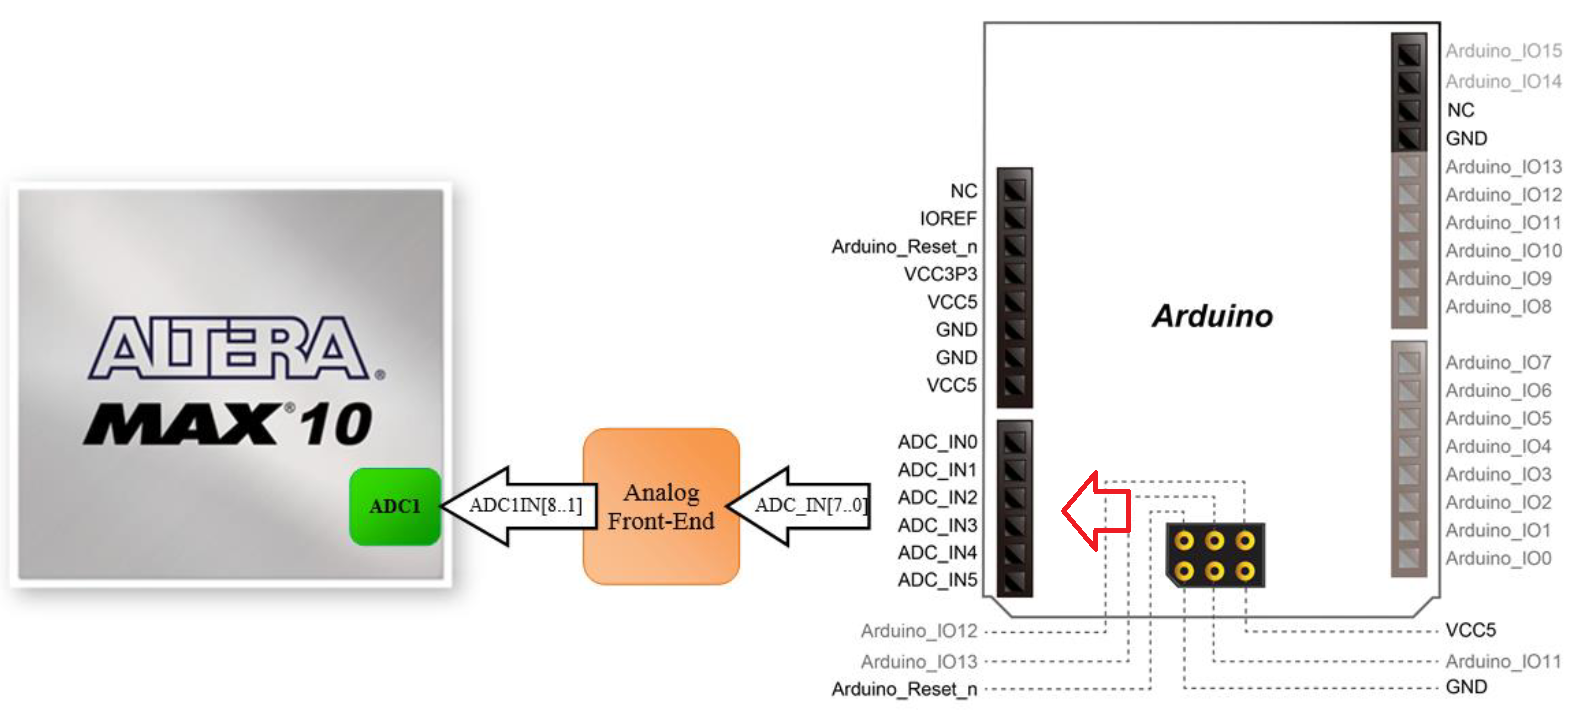
\includegraphics[width=15cm]{SAUER/Grafiken/ADC_Arduino_Pins.PNG}
\caption{Blockschaltbild}
\label{ADC_Blockschaltbild}
\end{center}
\end{figure}
Das "analog Front-End"enthhält einen Vorverstärker, realisiert mittels OPV, der grundsätzlich die Aufgabe hat die Spannung zu halbieren. Somit werden die maximal zulässigen 5V auf 2,5V heruntergeregelt, welche die Referenzspannung des ADCs ist und diesen so nicht übersteuert. Die Transitfrequenz des MCP6244 liegt bei 550kHz. Bei 10MHz geht sich eine Verstärkung von 0,5 knapp aus, was jedoch wenig Bedeutung hat, da die Frequenz der Eingangssignale, aufgrund der Abtastrate von 10MSa/s, ohnehin kleiner sein muss. \\Wie in dem Schaltplanausschnitt (aus FPGA-Schaltplan: \ref{Schaltplan_FPGA}) in Abbildung \ref{Front-End_Schaltung} zu sehen, sind auch Kondensatoren vorhanden. Das Verhalten im Frequenzbereich wurde mithilfe von LtSpice analysiert. Da der orginale OPV im Simulationsprogramm nicht spezifiziert ist, wurde der sehr ähnliche AD8038 verwendet.
\begin{figure}[!h]
\begin{center}
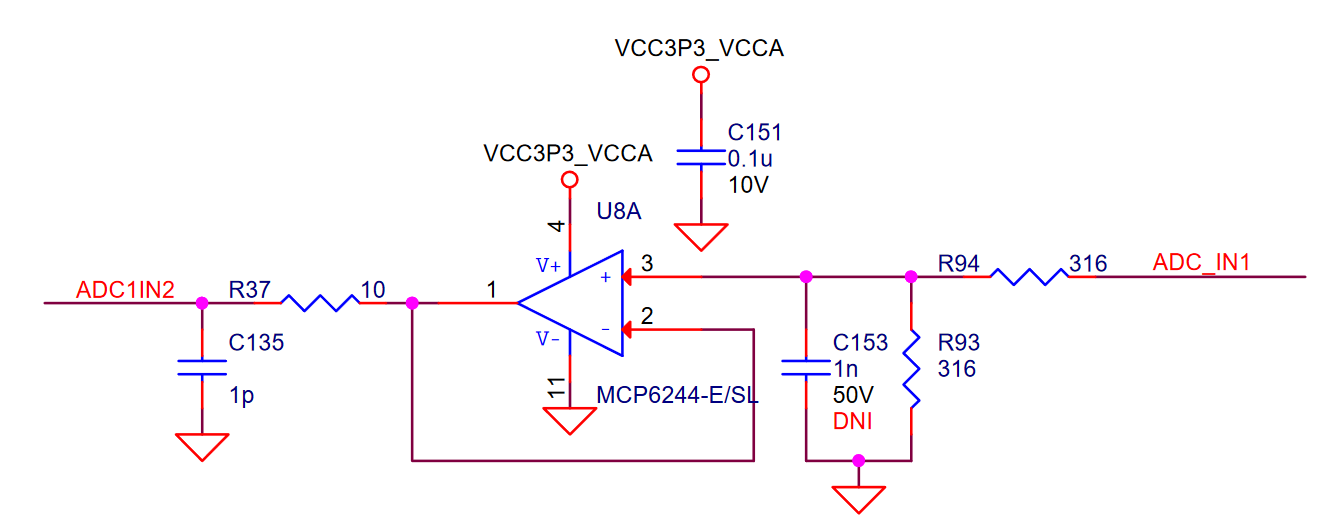
\includegraphics[width=15cm]{SAUER/Grafiken/ADC_Front-End.PNG}
\caption{analog Front-End Ch1}
\label{Front-End_Schaltung}
\end{center}
\end{figure}
\begin{figure}[!h]
\begin{center}
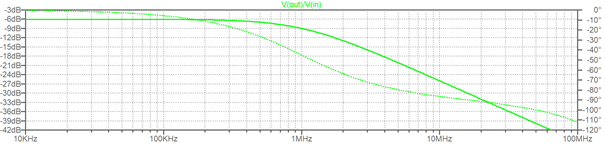
\includegraphics[width=15cm]{SAUER/Grafiken/ADC_Front-End_Bode.PNG}
\caption{Bodediagramm Vorverstärker}
\label{Front-End_Bode}
\end{center}
\end{figure}
\\Im Bodediagramm (Figure: \ref{Front-End_Bode}) ist die Verstärkung von $\frac{1}{2} = -6dB$ gut zu erkennen. Der Abfall von -20 dB pro Dekade beweißt die 1. Ordnung. Die Grenzfrequenz ($hier bei -9dB$) liegt bei 997kHz. Das ist locker ausreichend, da die Frequenz der Eingangssignale aufgrund der Abtastrate von 10MSa/s sowieso niedriger ist.
\subsubsection{VHDL Implementierung}
Es wurde mit verschiedenen IP-Cores von Quartus versucht die ADCs anzusteuern.  Eine Implementierung mit dem IP-Core "Modular ADC core Intel FPGA IP" über das "Avalon"-Interface wurde probiert, schlug jedoch fehl, da der "Fitter" von Quartus Prime nicht für eine Ansteuerung ohne Nios-Prozessor ausgelegt ist.
\textbf{Fazit:} Die internen ADCs im DE10-Lite Board können nur mit einem eigebetteten Nios Prozessor verwendet werden.